
\section{Network performance}

Units of measurement in this course (Must use these units in assignments):

\textbf{Data Size}: [KMG][bB]: $K=2^{10}, M=2^{20}, G=2^{30}$

\textbf{Data Rates}: [KMB]bps: $K=10^3, M=10^6, G=10^9$

\subsection{Network metrics}

\subsubsection{Rate metrics}

\begin{knBox}
    {Bandwidth}

    (Theoretical) Maximum rate of data transfer across a given path.

    \begin{itemize}
        \item \textbf{Useful for:} Streaming
        \item \textbf{Not useful for:} Live chat, surfing web, online games
    \end{itemize}
\end{knBox}

\begin{knBox}
    {Throughput}

    Actual rate of successful data transfer:

    \[\text{Throughput} = \frac{\text{Total data transferred (bits)}}{\text{Time taken (seconds)}}\]
\end{knBox}

\begin{knBox}
    {Goodput}

    Does not include headers, encodings, loss data and retransmissions.

    Depends on context and application-layer protocol.

    \[ \text{Goodput} = \frac{\text{Useful data transferred (bits)}}{\text{Time taken (seconds)}} \]

    \tcblower

    \textit{The goodput of transferring 10MB data with additional 1MB data over 12 seconds in Mbps is:} $10 \times 8 \times 2^{20} \div 12 \div 10^6 = 6.99$ Mbps
\end{knBox}

\subsubsection{Time metrics}

\begin{knBox}
    {Latency}

    Delay from when data is sent to when it is received.
\end{knBox}

\begin{knBox}
    {Round Trip Time (RTT)}

    [Latency for message + latency for response + processing time] Latency for sending data and receiving a response.
\end{knBox}

\begin{knBox}
    {Jitter}

    Variation in latency and/or RTT.
\end{knBox}

\subsection{Delay}

\subsubsection{Types of delay}



\begin{definition}
    {Traffic Intensity}

    How busy a link is:

    \[\text{Traffic Intensity} = \frac{L \times a}{R}\]

    Where $L$ is the packet length (bits), $a$ is the average packet arrival rate (packets/sec), and $R$ is the transmission rate (bps).

    \begin{itemize}
        \item If traffic intensity $> 1$, the queue will grow and the router will need to drop a significant number of packets
        \item If traffic intensity $\approx 1$, the router will \textbf{still} drop packets as traffic is \textbf{bursty} (don't arrive uniformly)
    \end{itemize}

    \tcblower

    \textit{Suppose a router is connected to a 1Mbps link. The router receives an average of
        100 packets per second, averaging 500 bytes per packet. What is the traffic
        intensity?}


    TODO: VERIFY

    \[L = 500 \times 8 = 4000 \text{ bits}, a = 100 \text{ packets/sec}, R = 1 \times 10^6 \text{ bps}\]
\end{definition}

\begin{knBox}
    {Processing delay}

    Examine packet to decide where to direct it
\end{knBox}

\begin{knBox}
    {Queuing delay}

    Waiting time to get access to the link. Each link has a queue where packets wait to be transmitted.

    The higher the \textbf{traffic intensity}, the link is busier, and higher probability that there is one or more packets in the queue.

    Assuming packets arrive at an exponential rate, total delay is:

    \[D = \frac{S}{1-U}\]

    Queing delay is:

    \[t_{\text{queue}} = D - S = \frac{S}{1-U} - S = \frac{U \times S}{1-U}\]

    Where $S$ is average service time when server is idle, and $U$ is the traffic intensity (server utilization).
\end{knBox}

\begin{knBox}
    {Transmission delay}

    Time to actually write the packet onto the medium:

    \[t_{\text{trans}} = \frac{\text{Packet size (bits)}}{\text{Transfer rate (bps)}}\]
\end{knBox}

\begin{knBox}
    {Propagation delay}

    Time spent to move each bit from source to destination on the transmission medium (similar to latency):

    \[t_{\text{prop}} = \frac{\text{Distance (m)}}{\text{Propagation speed (m/s)}}\]
\end{knBox}

\begin{knBox}
    {End-to-end delay}

    Sum of all sources of delay
\end{knBox}

\begin{center}
    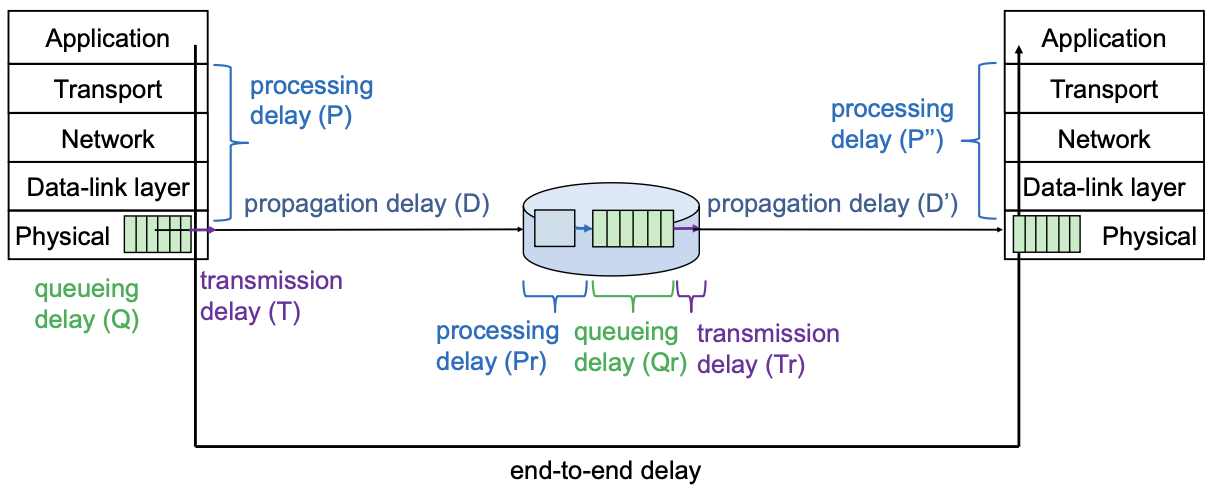
\includegraphics[width=0.8\textwidth]{./images/m02-l02-1.png}
\end{center}